% Generated by pysimcount.pfseeds -- do not edit; regenerate instead.
% figure: B-all-by-formula -- Every formula at measured r; median over seeds [1, 2, 3, 4, 5, 6, 7, 8, 9, 10], bars = min..max
% metric=cnot gatebase=cz merged
% seed 1: git_commit=01d3c275ceae2840002bd1aaea68f59b987c4975 git_dirty=False
% seed 2: git_commit=01d3c275ceae2840002bd1aaea68f59b987c4975 git_dirty=False
% seed 3: git_commit=01d3c275ceae2840002bd1aaea68f59b987c4975 git_dirty=False
% seed 4: git_commit=01d3c275ceae2840002bd1aaea68f59b987c4975 git_dirty=False
% seed 5: git_commit=01d3c275ceae2840002bd1aaea68f59b987c4975 git_dirty=False
% seed 6: git_commit=01d3c275ceae2840002bd1aaea68f59b987c4975 git_dirty=False
% seed 7: git_commit=01d3c275ceae2840002bd1aaea68f59b987c4975 git_dirty=False
% seed 8: git_commit=01d3c275ceae2840002bd1aaea68f59b987c4975 git_dirty=False
% seed 9: git_commit=01d3c275ceae2840002bd1aaea68f59b987c4975 git_dirty=False
% seed 10: git_commit=01d3c275ceae2840002bd1aaea68f59b987c4975 git_dirty=False
% derived: B-all-by-formula.tex with Lie-Trotter S1 removed by pysimcount.figdrop (Lie-Trotter S1 alone spans 43% of the original y-axis); removed legends: Lie-Trotter S1; source_sha256=48dcbe5c331a59c5423ea8a08e2f0157836167fc4205585ed15d63626a78ea1f
% derived: B-all-by-formula-no-lie-trotter.tex restyled by pysimcount.figuniform: extrapolated points (r from power-law fit) drawn in their series' measured style, style-key legend entries removed; extrapolated n = [13, 20]; source_sha256=0daae01046ae6f50360b1df223234c005d76cc113769698648baf6ef82eff425
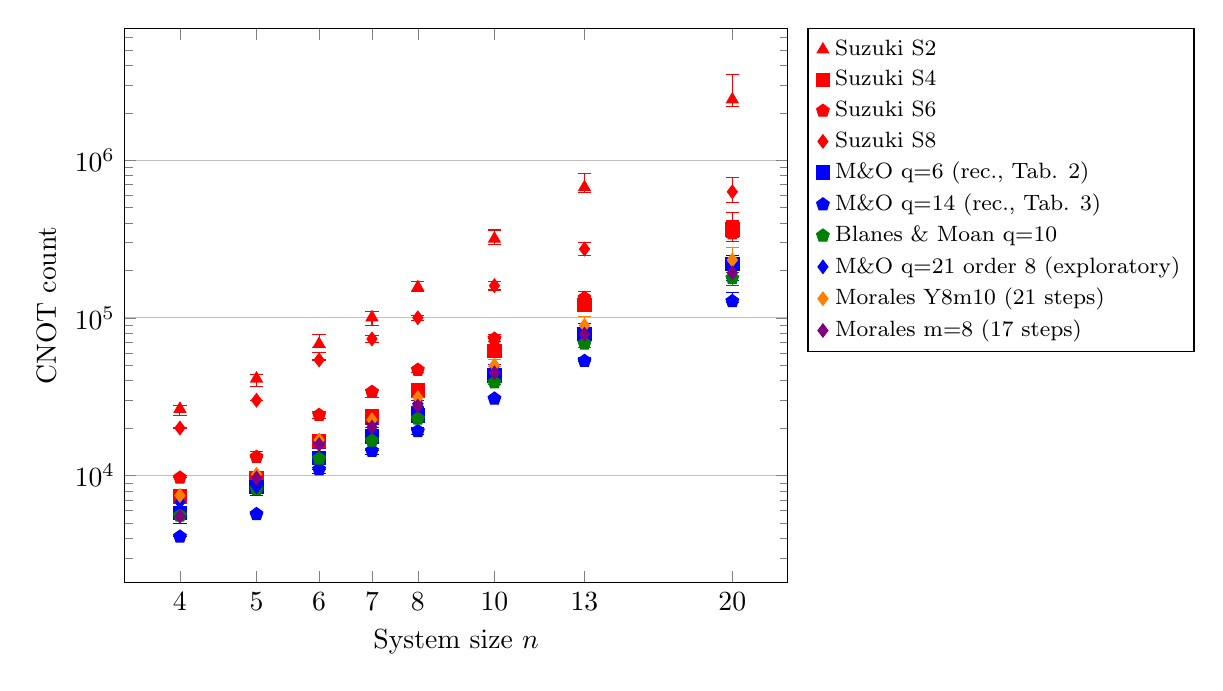
\begin{tikzpicture}
  \begin{loglogaxis}[
    width=10cm,
    xlabel={System size $n$},
    ylabel={CNOT count},
    xtick={4,5,6,7,8,10,13,20},
    xticklabels={4,5,6,7,8,10,13,20},
    ymajorgrids=true,
    legend pos=outer north east,
    legend cell align=left,
    legend style={font=\footnotesize},
  ]
    \addplot[only marks, red, mark=triangle*, mark size=2.4pt, mark options={solid, fill=red}, error bars/.cd, y dir=both, y explicit, error bar style={red}] coordinates {
      (4,26460) += (0,1500) -= (0,2300)
      (5,41200) += (0,2750) -= (0,4250)
      (6,68250) += (0,10230) -= (0,3150)
      (7,100765) += (0,9555) -= (0,10955)
      (8,156440) += (0,13400) -= (0,8360)
      (10,317650) += (0,43350) -= (0,26450)
    };
    \addlegendentry{Suzuki S2}
    \addplot[only marks, red, mark=triangle*, mark size=2.4pt, mark options={solid, fill=red}, forget plot, error bars/.cd, y dir=both, y explicit, error bar style={red}] coordinates {
      (13,673790) += (0,149630) -= (0,46410)
      (20,2428200) += (0,1074200) -= (0,230000)
    };
    \addplot[only marks, red, mark=square*, mark size=2.4pt, mark options={solid, fill=red}, error bars/.cd, y dir=both, y explicit, error bar style={red}] coordinates {
      (4,7392) += (0,168) -= (0,0)
      (5,9660) += (0,420) -= (0,210)
      (6,16632) += (0,1260) -= (0,756)
      (7,23961) += (0,2205) -= (0,1323)
      (8,34608) += (0,1344) -= (0,1344)
      (10,61530) += (0,5670) -= (0,1470)
    };
    \addlegendentry{Suzuki S4}
    \addplot[only marks, red, mark=square*, mark size=2.4pt, mark options={solid, fill=red}, forget plot, error bars/.cd, y dir=both, y explicit, error bar style={red}] coordinates {
      (13,120939) += (0,17199) -= (0,7917)
      (20,363720) += (0,102480) -= (0,42000)
    };
    \addplot[only marks, red, mark=pentagon*, mark size=2.4pt, mark options={solid, fill=red}, error bars/.cd, y dir=both, y explicit, error bar style={red}] coordinates {
      (4,9696) += (0,0) -= (0,0)
      (5,13130) += (0,1010) -= (0,0)
      (6,24240) += (0,1212) -= (0,1212)
      (7,33936) += (0,1414) -= (0,2828)
      (8,46864) += (0,1616) -= (0,1616)
      (10,73730) += (0,5050) -= (0,3030)
    };
    \addlegendentry{Suzuki S6}
    \addplot[only marks, red, mark=pentagon*, mark size=2.4pt, mark options={solid, fill=red}, forget plot, error bars/.cd, y dir=both, y explicit, error bar style={red}] coordinates {
      (13,133926) += (0,13130) -= (0,7878)
      (20,343400) += (0,68680) -= (0,36360)
    };
    \addplot[only marks, red, mark=diamond*, mark size=2.4pt, mark options={solid, fill=red}, error bars/.cd, y dir=both, y explicit, error bar style={red}] coordinates {
      (4,20040) += (0,0) -= (0,0)
      (5,30060) += (0,0) -= (0,0)
      (6,54108) += (0,6012) -= (0,0)
      (7,73647) += (0,3507) -= (0,3507)
      (8,100200) += (0,4008) -= (0,4008)
      (10,160320) += (0,10020) -= (0,10020)
    };
    \addlegendentry{Suzuki S8}
    \addplot[only marks, red, mark=diamond*, mark size=2.4pt, mark options={solid, fill=red}, forget plot, error bars/.cd, y dir=both, y explicit, error bar style={red}] coordinates {
      (13,273546) += (0,26052) -= (0,26052)
      (20,631260) += (0,150300) -= (0,90180)
    };
    \addplot[only marks, blue, mark=square*, mark size=2.4pt, mark options={solid, fill=blue}, error bars/.cd, y dir=both, y explicit, error bar style={blue}] coordinates {
      (4,5800) += (0,200) -= (0,800)
      (5,8500) += (0,250) -= (0,1000)
      (6,12900) += (0,300) -= (0,600)
      (7,17675) += (0,875) -= (0,1225)
      (8,24000) += (0,2400) -= (0,1200)
      (10,43250) += (0,1750) -= (0,2750)
    };
    \addlegendentry{M\&O q=6 (rec., Tab. 2)}
    \addplot[only marks, blue, mark=square*, mark size=2.4pt, mark options={solid, fill=blue}, forget plot, error bars/.cd, y dir=both, y explicit, error bar style={blue}] coordinates {
      (13,78975) += (0,5525) -= (0,1625)
      (20,219500) += (0,21500) -= (0,8500)
    };
    \addplot[only marks, blue, mark=pentagon*, mark size=2.4pt, mark options={solid, fill=blue}, error bars/.cd, y dir=both, y explicit, error bar style={blue}] coordinates {
      (4,4104) += (0,0) -= (0,0)
      (5,5700) += (0,0) -= (0,0)
      (6,10944) += (0,0) -= (0,684)
      (7,14364) += (0,0) -= (0,798)
      (8,19152) += (0,912) -= (0,912)
      (10,30780) += (0,1140) -= (0,0)
    };
    \addlegendentry{M\&O q=14 (rec., Tab. 3)}
    \addplot[only marks, blue, mark=pentagon*, mark size=2.4pt, mark options={solid, fill=blue}, forget plot, error bars/.cd, y dir=both, y explicit, error bar style={blue}] coordinates {
      (13,53352) += (0,2964) -= (0,0)
      (20,127680) += (0,18240) -= (0,2280)
    };
    \addplot[only marks, green!50!black, mark=pentagon*, mark size=2.4pt, mark options={solid, fill=green!50!black}, error bars/.cd, y dir=both, y explicit, error bar style={green!50!black}] coordinates {
      (4,5576) += (0,328) -= (0,0)
      (5,8200) += (0,0) -= (0,410)
      (6,12792) += (0,0) -= (0,492)
      (7,16646) += (0,574) -= (0,574)
      (8,22960) += (0,1312) -= (0,1312)
      (10,38950) += (0,410) -= (0,1230)
    };
    \addlegendentry{Blanes \& Moan q=10}
    \addplot[only marks, green!50!black, mark=pentagon*, mark size=2.4pt, mark options={solid, fill=green!50!black}, forget plot, error bars/.cd, y dir=both, y explicit, error bar style={green!50!black}] coordinates {
      (13,68757) += (0,2665) -= (0,3731)
      (20,178760) += (0,14760) -= (0,18040)
    };
    \addplot[only marks, blue, mark=diamond*, mark size=2.4pt, mark options={solid, fill=blue}, error bars/.cd, y dir=both, y explicit, error bar style={blue}] coordinates {
      (4,6800) += (0,0) -= (0,0)
      (5,8500) += (0,850) -= (0,0)
      (6,16320) += (0,1020) -= (0,1020)
      (7,21420) += (0,1190) -= (0,1190)
      (8,28560) += (0,1360) -= (0,1360)
      (10,47600) += (0,3400) -= (0,1700)
    };
    \addlegendentry{M\&O q=21 order 8 (exploratory)}
    \addplot[only marks, blue, mark=diamond*, mark size=2.4pt, mark options={solid, fill=blue}, forget plot, error bars/.cd, y dir=both, y explicit, error bar style={blue}] coordinates {
      (13,82875) += (0,9945) -= (0,7735)
      (20,204000) += (0,44200) -= (0,30600)
    };
    \addplot[only marks, orange, mark=diamond*, mark size=2.4pt, mark options={solid, fill=orange}, error bars/.cd, y dir=both, y explicit, error bar style={orange}] coordinates {
      (4,7480) += (0,0) -= (0,0)
      (5,10200) += (0,0) -= (0,0)
      (6,16830) += (0,510) -= (0,510)
      (7,22610) += (0,1190) -= (0,0)
      (8,31280) += (0,1360) -= (0,1360)
      (10,50150) += (0,4250) -= (0,850)
    };
    \addlegendentry{Morales Y8m10 (21 steps)}
    \addplot[only marks, orange, mark=diamond*, mark size=2.4pt, mark options={solid, fill=orange}, forget plot, error bars/.cd, y dir=both, y explicit, error bar style={orange}] coordinates {
      (13,89505) += (0,12155) -= (0,5525)
      (20,232900) += (0,45900) -= (0,32300)
    };
    \addplot[only marks, violet, mark=diamond*, mark size=2.4pt, mark options={solid, fill=violet}, error bars/.cd, y dir=both, y explicit, error bar style={violet}] coordinates {
      (4,5520) += (0,0) -= (0,0)
      (5,9660) += (0,0) -= (0,0)
      (6,15732) += (0,0) -= (0,828)
      (7,20286) += (0,966) -= (0,0)
      (8,27600) += (0,2208) -= (0,0)
      (10,44850) += (0,2070) -= (0,690)
    };
    \addlegendentry{Morales m=8 (17 steps)}
    \addplot[only marks, violet, mark=diamond*, mark size=2.4pt, mark options={solid, fill=violet}, forget plot, error bars/.cd, y dir=both, y explicit, error bar style={violet}] coordinates {
      (13,78936) += (0,5382) -= (0,3588)
      (20,193200) += (0,30360) -= (0,11040)
    };
  \end{loglogaxis}
\end{tikzpicture}
